\chapter{Introduction}
\label{ch:intro}

\section{Context}
\label{sec:intro-context}

In September 2024 the University of Sheffield held its Festival of the Mind, and at one installation visitors were asked to type in how they felt. Whatever they typed went straight to DALL$\cdot$E, the model named in each file's provenance data, and the line drawing that came back, in black and white, went up on the screen for the visitor. There are \nTotal{} of these prompt--drawing records in all. They reached me when the project began in June 2026 as a folder of PNG files and a single JSON file of bare strings, without labels or metadata and with nothing to say who had typed what. The project specification offered a text strand and an image strand and left the focus to me.

Two features of the material shaped the work. First, the entries are short, and most of them are about the writer. The median length is four words, and 294 of the analysed records consist of one word only. The word ``happy'' by itself was typed \nHappy{} times, and other common entries are ``curious'', ``ok'', ``excited'' and ``good''. Many entries name more than one feeling at once, often feelings that pull against each other, as in ``tired but happy'' or ``tired proud happy'', and ``tired'' turns up inside many of the longer entries. A single label would lose part of what such an entry says. Second, every drawing is monochrome. The installation software appended a line-art instruction to each prompt (the instruction itself is not part of the data), so colour, which the literature treats as the main carrier of emotion in generated images \cite{alvarado2025texttoimage}, is missing from all \nTotal{} drawings. Whatever an automatic reader can recover from them has to come from line, posture, faces and composition.

The interface accepted any text at all. Some entries are not about a feeling at all: ``pigs'', which appears repeatedly, ``mickey mouse'', ``disney characters'', ``i like football'', and questions put to the machine such as ``how can a circle be squared''. Nothing ties a record to a person, so someone could have typed once or come back several times, and how many people contributed is unknown. Since \nRepeats{} of the \nAnalysed{} records repeat an earlier prompt, the count of contributors is at most \nDistinct{}, the number of distinct prompts. Every count in this dissertation is therefore a count of records. Figure~\ref{fig:examples} gives six records in the form used throughout this dissertation, the visitor's words with any personal name replaced by a placeholder, next to the drawing made from them.

\begin{figure}[htbp]
\centering
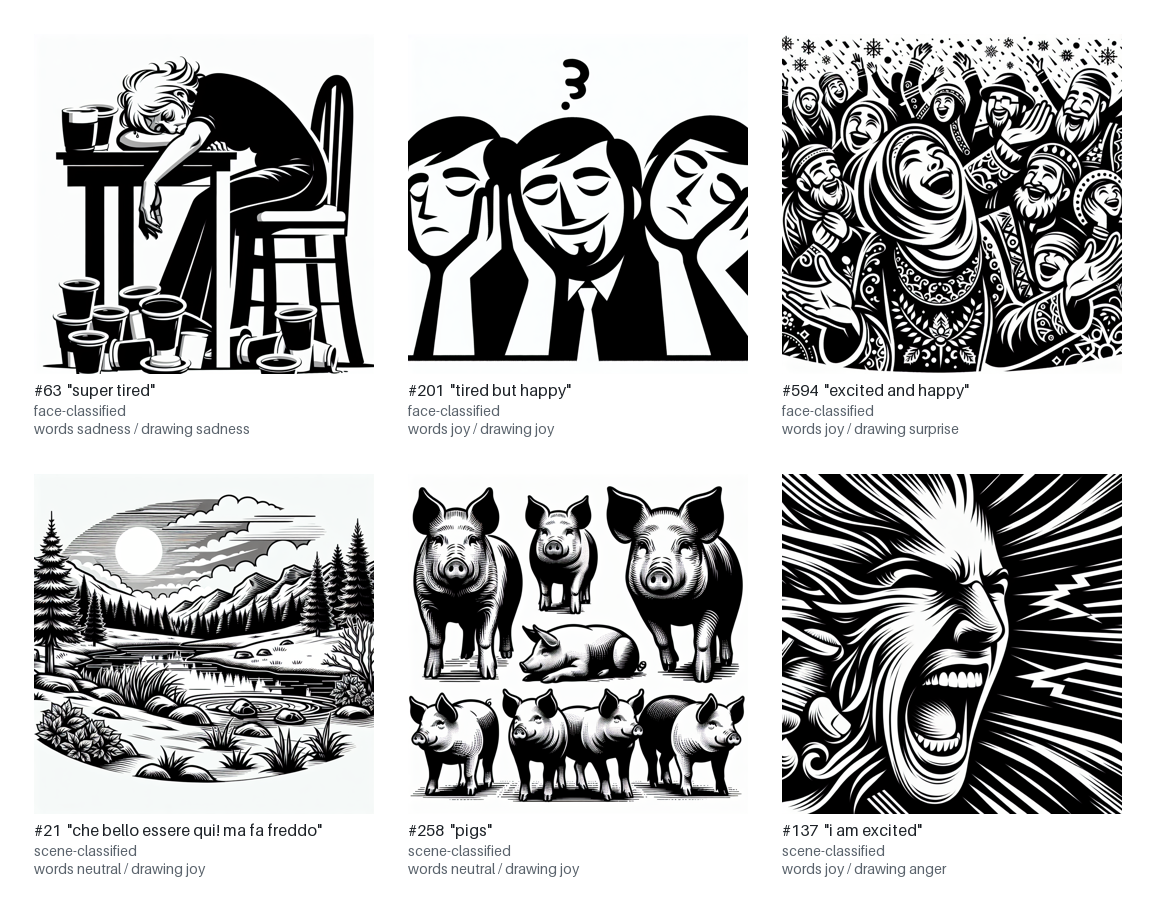
\includegraphics[width=\textwidth]{examples}
\caption{Six records as they appear throughout this dissertation. Under each drawing are the record number, the prompt as typed, the class the describer assigned (face or scene, Section~\ref{sec:method-pipeline}) and the family returned by each of the two readers. The demonstrator examples (Section~\ref{sec:method-demo}) are records 63 and 201. In record 21 the drawing is of mountains, the describer reported no people, and its expression answer was still ``smiling''; Section~\ref{sec:results-describer} reports how often that happens.}
\label{fig:examples}
\end{figure}

\section{The question}
\label{sec:intro-question}

If someone types something about how they feel and an image generator draws it, how far does the emotion read from the words agree with the emotion read from the drawing? That is the research question, and the data limit how it can be answered. Nobody rated these drawings, and the only record of what a visitor meant is what the visitor typed. Each side therefore gets an automatic reader in place of a person. A language model assigns the prompt an emotion, and a second reader does the same for the drawing by first putting it into words and then reading those words. All the numbers reported here are agreement between those two readings. What a person looking at a drawing would see is a separate question that needs human raters, and Chapter~\ref{ch:conclusion} lists that study as further work.

The design follows a direction my supervisor gave at a meeting at the end of July. Dr Chen is a psychologist who works on facial expressions, and her point was that scoring a drawing as a hit or a miss against a label is too crude for emotion. Two people looking at the same face will often not agree about what it is doing, and the models are noisy on top of that. The labels overlap as well. Cowen and Keltner \cite{cowen2017self} found 27 categories in self-reported experience, joined to one another by continuous gradients, and on Russell's circumplex \cite{russell1980circumplex, posner2005circumplex} ``happy'' lies a short distance from ``excited'' on the valence--arousal plane. If a visitor typed ``happy'' and the drawing is read as excited, counting that as a complete miss throws away most of what this corpus has to offer. So the project asks how similar two readings are, and it never scores a drawing on whether it matches a label. Dr Chen asked for this similarity framing to be named as the novel element of the work.

In place of the hit-or-miss score there are four measures arranged as a ladder, from loose to strict, and each is compared with what comes out when drawings are paired with prompts at random. Chapter~\ref{ch:method} defines them. Valence--arousal similarity is the loosest and family agreement, which needs the two top families to coincide, is the strictest; top-3 soft overlap and valence-sign agreement sit between them. The chance reference is needed because the loosest measure does not start at zero. Valence--arousal similarity has a floor of 0.412 on a scale whose top is 1, and a random pairing of drawings with prompts already scores about \FullNeuVaNull{}, so a value that looks respectable at first sight can sit below chance. I ran into this while building the demonstrator, when a value that looked fine on screen was in fact under the random-pairing mean.

\section{Aims and objectives}
\label{sec:intro-aims}

The aim is to measure how closely two automatic readers, one reading the visitor's words and the other the drawing, agree about the emotion in a record, with each value set against its chance level, and to describe the instrument well enough that its weak points are on record. There are eight objectives.

\begin{enumerate}
\item Build the image side as a describe-then-extract pipeline, in which a vision model answers factual questions about the picture and a separate text model reads an emotion from those answers, so that the vision model is never asked about emotion.
\item Define the four-rung similarity ladder and the random-pairing null, so that no value is reported without its chance level.
\item Measure agreement on the full corpus and then separately on the two splits Dr Chen asked for: emotional prompts against neutral-labelled ones, and face-classified drawings against scene-classified ones.
\item Put the face/scene difference to a formal test, and check that the headline results are not an artefact of the repeated prompts.
\item Run a like-for-like comparison between describe-then-extract and a direct CLIP reader, with both given the same records, the same prompt-side readings and the same measures.
\item Turn the repeated prompts into a consistency measurement, asking how far drawings made from one and the same prompt are given the same family by the image reader.
\item Audit the instrument. The checks are a control audit of the neutral-labelled prompts, an audit of the describer's answers, a taxonomy of the strongest disagreements by failure mode, a single-coder check on a blind sample of drawings, and an ablation over the description template.
\item Release the toolkit in a reproducible form, with the headline numbers pinned by tests and a demonstrator that runs the real models.
\end{enumerate}

\section{Contributions}
\label{sec:intro-contributions}

Very little of the software is new in itself. The prompt side uses RoBERTa fine-tuned on GoEmotions, the image side uses a visual question-answering model followed by a natural-language-inference model, and the inference relies on textbook procedures such as the clustered bootstrap and the permutation test. The new parts are the object of study and the question put to it, the practice of setting every answer against its chance level, the consistency experiment, and the audits.

The material is new because nobody gave the visitors a list of emotions to pick from or a template to fill in, and what they typed is mostly short self-reports from members of the public, many naming more than one feeling, each drawn as a line drawing with no colour in it. The closest prior study is by Lomas and colleagues \cite{lomas2024improved}. Their design differs on several points: ten emotions from a fixed list, each generated on a person or a robot, in colour, and scored by human raters. None of the 73 papers retained for the review in Chapter~\ref{ch:lit} measures agreement between the emotion read from a short, mixed self-report and the emotion read from a colour-free drawing made of it.

For each record the question is whether the two readings agree end to end, and it is answered with the ladder set against its null. Because \nRepeats{} records repeat a prompt and cannot be treated as independent, the intervals are clustered on prompt groups, and the one contrast the design was built around, face-classified against scene-classified drawings, gets a formal permutation test. The repeated prompts also allow a consistency experiment. It needs the same words drawn more than once, which none of the studies reviewed in Chapter~\ref{ch:lit} had, and it measures how often the image reader gives the same family to a prompt drawn again.

The audits put numbers on the instrument's weak points: how far the image reading depends on a single word from the describer, what the describer answers when the drawing has no face in it, how many of the neutral-labelled prompts contain a plain affect word after all, and how many of the strongest disagreements can be traced to the generator as against the readers. Until the second audit in September the scene drawings looked as if they sat a little above chance. The template ablation in that audit removed that result (Chapter~\ref{ch:results}).

In practical terms the deliverables are the analysis code, the result tables over the \nAnalysed{} records, the demonstrator, a two-layer test suite and the audits themselves. The demonstrator is a small Flask application, run locally, that puts any analysed record or an uploaded image through the real models and reports all four measures against the chance levels the analysis uses. One test layer is a shell script that checks the environment, the corpus files and the cached model outputs, then runs the live pipeline over a few fresh images; the other pins each headline number to the JSON file behind it. Each statistic in the text is a LaTeX macro produced from those same result files. Re-running the analysis rewrites the numbers here without anyone retyping them.

\section{Overview of the report}
\label{sec:intro-overview}

The literature review in Chapter~\ref{ch:lit} goes through eight themes, from theories of emotion to how the public receives pictures made by AI, and closes by stating the gap the project sits in. Chapter~\ref{ch:method} covers the corpus and its pre-processing, then the two readers, then the ladder with its null and the inference procedures, then each analysis, the demonstrator and the alternatives I tried first and dropped. The numbers, with their tables and figures, are in Chapter~\ref{ch:results}. Interpretation is held over to Chapter~\ref{ch:discussion}, which sets out what the results do and do not establish, why the weakest part of the chain is the describer, and how the findings sit next to earlier work. Chapter~\ref{ch:conclusion} closes with further work in the order the evaluation points to. Three appendices follow. Appendix~\ref{app:repro} gives the layout of the repository, the order in which the scripts run and the pinned environment. Appendix~\ref{app:instruments} collects the fixed strings the pipeline depends on: the five describer questions, the description template, the hypothesis string, the expression-word list, the category-to-family map, the circumplex centroids, the coder's instructions and the redaction procedure. The record of supervision meetings is Appendix~\ref{app:supervision}.
